\documentclass[letter]{article}

\usepackage[spanish]{babel}
\usepackage[margin=1in]{geometry}
\usepackage{amsmath}
\usepackage{amsthm}
\usepackage{amssymb}
\usepackage[utf8]{inputenc}
\usepackage{graphicx, color}
\usepackage{algorithm}
\usepackage{algpseudocode}
\usepackage{mathrsfs}
% Cambiar el estilo de las listas
\renewcommand{\labelitemi}{$\bullet$}

% Some definitions
\floatname{algorithm}{Algoritmo}

% Author info
\title{Escritura del problema del ordenamiento de datos}
\author{Alejandro Morales Contreras$^1$}
\date{
	$^1$Departamento de Ingeniería de Sistemas, Pontificia Universidad Javeriana\\Bogotá,  Colombia \\
	\texttt{a.moralesc@javeriana.edu.co}\\~\\
	\today
}

\begin{document}
\maketitle
	
\begin{abstract}
En este documento se presenta la formalización del problema de ordenamiento de datos, junto con la descripción de tres algoritmos que lo solucionan. Además, se presenta un análisis experimental de la complejidad de esos tres algoritmos.
\textbf{Palabras clave:} ordenamiento, algoritmo, formalización, experimentación, complejidad.
\end{abstract}

\tableofcontents
	
\section{Introducción} \label{intro}
Los algoritmos de ordenamiento de datos son muy útiles en una cantidad considerable de algoritmos que requieren orden en los datos que serán procesados. En este documento se presentan tres de ellos, con el objetivo de mostrar: la formalización del problema (sección \ref{formalizacion}), la escritura formal de tres algoritmos (sección \ref{algoritmos}) y un análisis experimental de la complejidad de cada uno de ellos (sección \ref{experimentos}).

\section{Formalización del problema} \label{formalizacion}
Cuando se piensa en el {\it ordenamiento de números} la solución inmediata puede ser muy simplista: inocentemente, se piensa en ordenar números. Sin embargo, con un poco más de reflexión, hay tres preguntas que pueden surgir:
\begin{enumerate}
  \item ¿Cuáles números?
  \item ¿Cómo se guardan esos números en memoria?
  \item ¿Solo se pueden ordenar números?
\end{enumerate}

Recordemos que los números pueden ser naturales ($\mathbb{N}$), enteros ($\mathbb{Z}$), racionales o quebrados ($\mathbb{Q}$), irracionales ($\mathbb{I}$) y complejos ($\mathbb{C}$). En todos esos conjuntos, se puede definir la relación de {\it orden parcial} $a<b$.

Esto lleva a pensar: si se puede definir la relación de orden parcial $a<b$ en cualquier conjunto $\mathbb{T}$, entonces se puede resolver el problema del ordenamiento con elementos de dicho conjunto.

\subsection{Definición del problema del ``ordenamiento de datos''} \label{problema}
Así, el problema del ordenamiento se define a partir de:
  \begin{enumerate}
    \item una secuencia $S$ de elementos $a\in \mathbb{T}$ y
    \item una relación de orden parcial $a<b~\forall a,b\in \mathbb{T}$
  \end{enumerate}
producir una nueva secuencia $S'$ cuyos elementos contiguos cumplan con la relación $a<b$.
\begin{itemize}
    \item Entradas:
    \begin{itemize}
        \item $S = \left< a_i \in \mathbb{T} \right> ~ | ~ 1\le i \le n$.
        \item $a<b \in \mathbb{T} \times \mathbb{T}$, una relación de orden parcial.
    \end{itemize}
    \item Salidas:
    \begin{itemize}
        \item $S' = \left< e_i \in S m\right> ~ | ~ e_i < e_{i+1} \forall i \in \left[1,n\right)$.
    \end{itemize}
\end{itemize}

\section{Algoritmos de solución} \label{algoritmos}
\subsection{Burbuja ``inocente''} \label{algoritmos:inocente}
La idea de este algoritmo es: comparar todos las parejas de elementos adyacentes e intercambiarlos si no cumplen con la relación de orden parcial $<$.

\begin{algorithm}[!htb]
\caption{Ordenamiento por burbuja ``inocente''.}
\begin{algorithmic}[1]
\Require $S=\left< s_i \in \mathbb{T} \right> \land a<b \in \mathbb{T} \times \mathbb{T}$
\Ensure $S$ será cambiado por $S' = \left< e_i \in S  ~ | ~ e_i < e_{i+1} \forall i \in \left[1,n\right)\right>$
\Procedure{NaiveBubbleSort}{$S$}
  \For{$i \leftarrow 1~\mathbf{to}~|S|$}
    \For{$j \leftarrow 1~\mathbf{to}~|S|-1$}
      \If{$s_{j+1}<s_j$}
        \State \Call{Swap}{$s_j,s_{j+1}$}
      \EndIf
    \EndFor
  \EndFor
\EndProcedure
\end{algorithmic}
\end{algorithm}

\subsubsection{Análisis de complejidad} \label{algoritmos:inocente:complejidad}

Por inspección de código: hay dos ciclos {\it para-todo} anidados que, en el peor de los casos, recorren todo la secuencia de datos; entonces, este algoritmo es $O(|S|^2)$.

\subsubsection{Invariante} \label{algoritmos:inocente:invariante}

Después de cada iteración controlada por el contador $i$, los $i$ elementos más grandes quedan al final de la secuencia.

\begin{enumerate}
    \item Inicio: $i=0$, la secuencia vacía está ordenada.
    \item Iteración: $1 \le i<|S|$, si se supone que los $i-1$ elementos más grandes ya están en su posición, entonces la nueva iteración llevará los $i$-ésimo elemento a su posición adecuada.
    \item Terminación: $i=|S|$, los $|S|$ elementos más grandes están en su posición, entonces la secuencia está ordenada.
\end{enumerate}

\subsection{Burbuja ``mejorado''} \label{algoritmos:mejorado}

La idea de este algoritmo es: comparar todos las parejas de elementos adyacentes e intercambiarlos si no cumplen con la relación de orden parcial $<$, con la diferencia que las comparaciones se detienen en el momento que se alcanzan los elementos más grandes que ya están en su posición final.

\begin{algorithm}[!htb]
\caption{Ordenamiento por burbuja ``mejorado''.}
\begin{algorithmic}[1]
\Require $S=\left< S_i \in \mathbb{T} \right> \land a<b \in \mathbb{T} \times \mathbb{T}$
\Ensure $S$ será cambiado por $S' = \left< e_i \in S  ~ | ~ e_i < e_{i+1} \forall i \in \left[1,n\right)\right>$
\Procedure{ImprovedBubbleSort}{$S$}
  \For{$i \leftarrow 1~\mathbf{to}~|S|$}
    \For{$j \leftarrow 1~\mathbf{to}~|S|-i$} \Comment{Mejora: parar cuando se encuentren los elementos más grandes.}
      \If{$s_{j+1}<s_j$}
        \State \Call{Swap}{$s_j,s_{j+1}$}
      \EndIf
    \EndFor
  \EndFor
\EndProcedure
\end{algorithmic}
\end{algorithm}

\subsubsection{Análisis de complejidad} \label{algoritmos:mejorado:complejidad}

Por inspección de código: hay dos ciclos {\it para-todo} anidados que, en el peor de los casos, recorren todo la secuencia de datos; entonces, este algoritmo es $O(|S|^2)$.

\subsubsection{Invariante} \label{algoritmos:mejorado:invariante}

Después de cada iteración controlada por el contador $i$, los $i$ elementos más grandes quedan al final de la secuencia.

\begin{enumerate}
    \item Inicio: $i=0$, la secuencia vacía está ordenada.
    \item Iteración: $1 \le i<|S|$, si se supone que los $i-1$ elementos más grandes ya están en su posición, entonces la nueva iteración llevará los $i$-ésimo elemento a su posición adecuada.
    \item Terminación: $i=|S|$, los $|S|$ elementos más grandes están en su posición, entonces la secuencia está ordenada.
\end{enumerate}

\subsection{Inserción} \label{algoritmos:insercion}

La idea de este algoritmo es: en cada iteración, buscar la posición donde el elemento que se está iterando quede en el orden de secuencia adecuado.

\begin{algorithm}[!htb]
\caption{Ordenamiento por inserción.}
\begin{algorithmic}[1]
\Require $S=\left< S_i \in \mathbb{T} \right> \land a<b \in \mathbb{T} \times \mathbb{T}$
\Ensure $S$ será cambiado por $S' = \left< e_i \in S m\right> ~ | ~ e_i < e_{i+1} \forall i \in \left[1,n\right)$
\Procedure{InsertionSort}{$S$}
  \For{$j \leftarrow 2~\mathbf{to}~|S|$}
    \State $k \leftarrow s_j$
    \State $i \leftarrow j - 1$
    \While{$0<i \land k < s_i$}
      \State $s_{i+1} \leftarrow s_i$
      \State $i \leftarrow i - 1$
    \EndWhile
    \State $s_{i+1} \leftarrow k$
  \EndFor
\EndProcedure
\end{algorithmic}
\end{algorithm}

\subsubsection{Análisis de complejidad} \label{algoritmos:insercion:complejidad}

Por inspección de código: hay dos ciclos (un {\it mientras-que} anidado dentro de un ciclo {\it para-todo}) anidados que, en el peor de los casos, recorren todo la secuencia de datos; entonces, este algoritmo es $O(|S|^2)$.

El ciclo interior, por el hecho de ser {\it mientras-que}, puede que en algunas configuraciones no se ejecute (i.e. cuando la secuencia ya esté ordenada); entonces, este algoritmo tiene una cota inferior $\Omega(|S|)$, dónde solo el {\it para-todo} recorre la secuencia.

\subsubsection{Invariante} \label{algoritmos:insercion:invariante}

Después de cada iteración $j$, los primeros $j$ siguen la relación de orden parcial $a<b$.

\begin{enumerate}
    \item Inicio: $j \le 1$, la secuencia vacía o unitaria está ordenada.
    \item Iteración: $2 \le j < |S|$, si se supone que los $j-1$ elementos ya están ordenados, entonces la nueva iteración llevará un nuevo elemento y los $j$ primeros elementos estarán ordenados.
    \item Terminación: $j=|S|$, los $|S|$ primeros elementos están ordenados, entonces la secuencia está ordenada.
\end{enumerate}

\section{Análisis experimental} \label{experimentos}

En esta sección se presentarán algunos los experimentos para confirmar los órdenes de complejidad de los tres algoritmos presentados en la sección \ref{algoritmos}.

\subsection{Secuencias aleatorias} \label{experimentos:aleatorias}

Acá se presentan los experimentos cuando los algoritmos se ejecutan con secuencias de entrada de orden aleatorio.

\subsubsection{Protocolo}
\begin{enumerate}
    \item Cargar en memoria un archivo de, al menos, 200Kb.
    \item Definir un rango $(b,e,s)\in\mathbb{N}^3$, donde: $b$ es un tamaño inicial, $e$ es un tamaño final y $s$ es un salto. Se generarán secuencias, a partir del archivo de entrada, de diferentes tamaños desde $b$ hasta $e$, adicionando cada vez $s$ elementos.
    \item Cada algoritmo se ejecutará 10 veces con cada secuencia y se guardará el tiempo promedio de ejecución.
    \item Se generan los gráficos necesarios para comparar los algoritmos.
\end{enumerate}

\subsection{Secuencias ordenadas} \label{experimentos:ordenadas}

Acá se presentan los experimentos cuando los algoritmos se ejecutan con secuencias de entrada ordenadas de acuerdo al orden parcial $a<b$.

\subsubsection{Protocolo}
\begin{enumerate}
    \item Definir un rango $(b,e,s)\in\mathbb{N}^3$, donde: $b$ es un tamaño inicial, $e$ es un tamaño final y $s$ es un salto. Se generarán secuencias aleatorias de diferentes tamaños desde $b$ hasta $e$, adicionando cada vez $s$ elementos.
    \item Se usará el algoritmo \texttt{sort(S)}, disponible en la librería básica de python, para ordenar dicha secuencia.
    \item Cada algoritmo se ejecutará 10 veces con cada secuencia ordenada y se guardará el tiempo promedio de ejecución.
    \item Se generan los gráficos necesarios para comparar los algoritmos.
\end{enumerate}

\subsection{Secuencias ordenadas invertidas} \label{experimentos:invertidas}

Acá se presentan los experimentos cuando los algoritmos se ejecutan con secuencias de entrada ordenadas de forma invertida de acuerdo al orden parcial $a<b$.

\subsubsection{Protocolo}
\begin{enumerate}
    \item Definir un rango $(b,e,s)\in\mathbb{N}^3$, donde: $b$ es un tamaño inicial, $e$ es un tamaño final y $s$ es un salto. Se generarán secuencias aleatorias de diferentes tamaños desde $b$ hasta $e$, adicionando cada vez $s$ elementos.
    \item Se usará el algoritmo \texttt{sort(S)}, disponible en la librería básica de python, para ordenar dicha secuencia.
    \item Cada algoritmo se ejecutará 10 veces con cada secuencia ordenada y se guardará el tiempo promedio de ejecución.
    \item Se generan los gráficos necesarios para comparar los algoritmos.
\end{enumerate}

\section{Resultados de los experimentos} \label{resultados}

Para la realización de los experimentos, se sigue el protocolo para cada tipo de secuencias que fueron definidas en la sección \ref{experimentos}. Los resultados de los experimentos esperan probar (o refutar) los análisis de complejidad realizados para cada uno de los algoritmos en la sección \ref{algoritmos}. \par

Para analizar estos resultados, se hace primeramente una inspección empírica de la gráfica resultante en donde se grafica el tamaño de la secuencia (número de elementos) contra el tiempo promedio que le toma a cada algoritmo ordenarla. Por ejemplo, para todos los algoritmos, el peor de los casos son secuencias aleatorias, las cuales representan una complejidad de $O(|S|^2)$. Se esperaría que la gráfica resultante fuera una parábola. \par

Cabe resaltar que, aunque los algoritmos tengan una complejidad equivalente, las gráficas no serán exactamente similares. Las optimizaciones que los algoritmos implementen podrán significar un crecimiento más lento que un algoritmo menos optimizado. Así mismo, la secuencia dada para el experimento también variará considerablemente el desempeño del algoritmo. Sin embargo, la medida de complejidad sigue siendo la adecuada para escoger el algoritmo. \par

Después de la inspección de la gráfica, es necesario confirmar más detalladamente si realmente los resultados prueban el análisis de complejidad. Una buena forma de confirmar esto es mediante una regresión de los datos. A excepción del algoritmo por inserción en el mejor de sus casos (una secuencia ordenada), todos los algoritmos presentan una complejidad de $O(|S|^2)$. Es por esto que una regresión cuadrática es la operación adecuada para confirmar los resultados. \par

La regresión cuadrática pretende ajustar una curva de la forma:

\[f(X) = aX^{2} + bX + c\]

donde $X$ representaría la variable independiente (tamaño de la secuencia) y $f(X)$ la variable dependiente (tiempo que toma ordenar la secuencia). Después de la regresión, se obtienen los coeficientes del polinomio $a$, $b$ y $c$. \par

La medida que se utiliza para determinar si la regresión se cumple es el coeficiente de determinación ($R^{2}$), el cual refleja que tan bien ajustado es el polinomio resultante a los datos de entrada. Esta se calcula así:

\[R^{2} = \frac{\sum_{n=1}^{N} (\hat{Y_n} - \Bar{Y})^2}{\sum_{n=1}^{N} (Y_n - \Bar{Y})^2} \]

en donde:

\begin{itemize}
    \item $N$ representa la cantidad de elementos o tamaño de la secuencia
    \item $\Bar{Y}$ representa la media de la variable dependiente de entrada
    \item $\hat{Y_n}$ representa $f(X_n)$ o el resultado de evaluar el polinomio de regresión en $X_n$
    \item $Y_n$ representa el n-ésimo dato de la variable dependiente de entrada
\end{itemize}

$R^2$ varía en el rango $(0,1)$ y a mayores medidas de este se espera una mayor confianza en que los resultados se asemejan a un polinomio cuadrático.\par

\subsection{Secuencias aleatorias} \label{resultados:aleatorias}

Para el experimento con secuencias aleatorias, se sigue el protocolo definido en la sección \ref{experimentos:aleatorias}, dando como rango $(b,e,s)$ los datos $(0,10000,100)$. Obtenidos los resultados, se genera el gráfico comparativo de los algoritmos presentado en la figura \ref{fig:grafica:aleatorias}.

\begin{figure}[!htb]
\centering
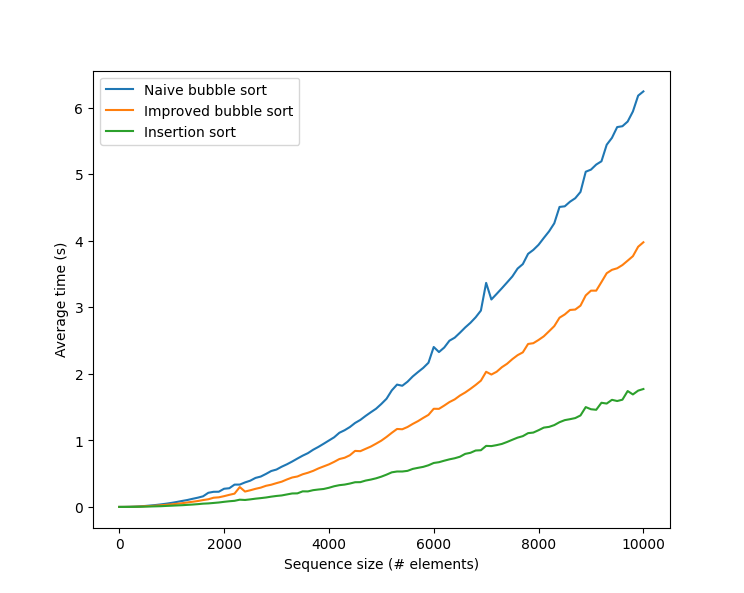
\includegraphics[scale=0.56]{img/plot_random.png}
\vspace{-1em}
\caption{Gráfica comparativa con secuencias aleatorias}
\label{fig:grafica:aleatorias}
\end{figure}

La inspección empírica de la gráfica parece revelar que los tres algoritmos siguen una parábola, cumpliendo con el análisis de complejidad. Así mismo, se resalta que el algoritmo de inserción tiene un mejor desempeño que los demás, mientras que el algorito de burbuja ``inocente'' tiene un peor desempeño que el resto. \par

Posteriormente, se realiza la regresión cuadrática y se obtienen los siguientes resultados: \par

\begin{table}[!ht]
\begin{tabular}{|l|r|r|r|r|}
\hline
Algoritmo        & \multicolumn{1}{c|}{$a$} & \multicolumn{1}{c|}{$b$} & \multicolumn{1}{c|}{$c$} & \multicolumn{1}{c|}{$R^2$} \\ \hline
Burbuja inocente & 6.19524e-08            & 3.15077e-06            & 1.04866e-03            & 0.9993555              \\ \hline
Burbuja mejorado & 3.94208e-08            & 2.43998e-06            & 1.05354e-03            & 0.9996105              \\ \hline
Inserción        & 1.75967e-08            & 3.64248e-06            & -2.70654e-03           & 0.9992336              \\ \hline
\end{tabular}
\end{table}

Como se puede ver, todos los algoritmos obtienen un $R^2 > 0,999$. Esto representa un ajuste bastante alto mediante la regresión cuadrática. Es posible confirmar que, con secuencias aleatorias, estos algoritmos tienen una complejidad de $O(|S|^2)$.

\subsection{Secuencias ordenadas} \label{resultados:ordenadas}

Para el experimento con secuencias aleatorias, se sigue el protocolo definido en la sección \ref{experimentos:ordenadas}, dando como rango $(b,e,s)$ los datos $(0,10000,100)$. Obtenidos los resultados, se genera el gráfico comparativo de los algoritmos presentado en la figura \ref{fig:grafica:ordenadas}.

\vspace{-1em}
\begin{figure}[!htb]
\centering
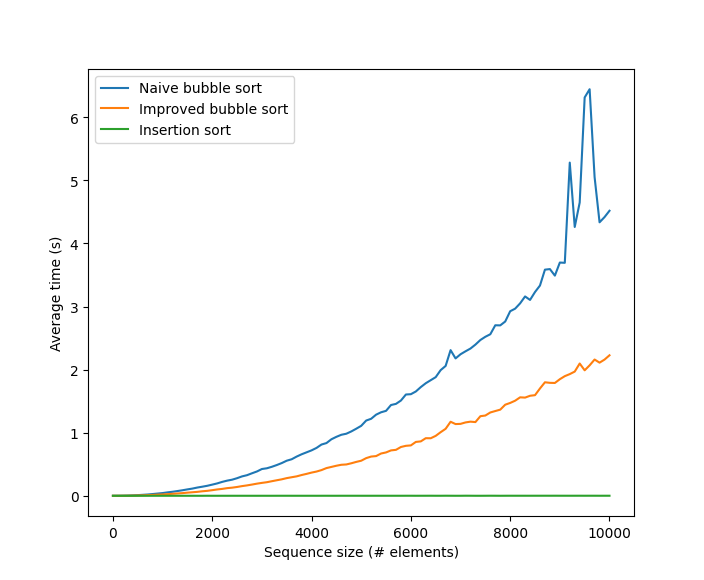
\includegraphics[scale=0.56]{img/plot_sorted.png}
\vspace{-1em}
\caption{Gráfica comparativa con secuencias ordenadas}
\label{fig:grafica:ordenadas}
\end{figure}

La inspección empírica de la gráfica parece revelar que ambos algoritmos burbuja siguen una parábola, pero el algoritmo por inserción parece ser una recta en $y=0$. Así mismo, el algoritmo de burbuja ``inocente'' sigue comportándose de la misma forma que en el anterior experimento (aunque con un picos que podrían ser explicados por la prioridad que el SO asigna a este proceso). Por su parte, el algoritmo de burbuja ``mejorado'' tiene un desempeño levemente mejor que en el anterior experimento. \par

Posteriormente, se realiza la regresión cuadrática y se obtienen los siguientes resultados: \par

\begin{table}[!ht]
\begin{tabular}{|l|r|r|r|r|}
\hline
Algoritmo        & \multicolumn{1}{c|}{$a$} & \multicolumn{1}{c|}{$b$} & \multicolumn{1}{c|}{$c$} & \multicolumn{1}{c|}{$R^2$} \\ \hline
Burbuja inocente & 6.04217e-08            & -1.11239e-04            & 1.24728e-01            & 0.9574511              \\ \hline
Burbuja mejorado & 2.21122e-08            & 6.39194e-06            & -9.27824e-03            & 0.9986932              \\ \hline
Inserción        & -7.54501e-08            & 9.294548e-08            & -9.51056e-06           & 0.7012384              \\ \hline
\end{tabular}
\end{table}

Analizando los resultados, los algoritmos de burbuja obtienen un $R^2 > 0,95$. Esto sigue representando un ajuste alto mediante regresión cuadrática (La disminución de la medida para la burbuja ``inocente'' puede ser explicada por el fenómeno del SO). Es posible confirmar que, con secuencias ordenadas, estos algoritmos tienen una complejidad de $O(|S|^2)$. \par

Por otro lado, el algoritmo de inserción no tiene un buen ajuste mediante regresión cuadrática. Esto se debe a que la cota inferior del algoritmo es $\Omega(|S|)$ y esta se presenta en el mejor de los casos del algoritmo (cuando la secuencia ya está ordenada). Se realiza entonces una regresión lineal de la forma $f(X) = aX + b$ y se obtiene: \par

\begin{table}[!ht]
\begin{tabular}{|l|r|}
\hline
$a$ & 8.54004e-08 \\ \hline
$b$ & 2.93870e-06 \\ \hline
$R^2$ & 0.7008665 \\ \hline
\end{tabular}
\end{table}

Como se evidencia por el valor de $R^2$, la confianza en que los datos representen una recta tampoco es muy grande. Sin embargo, dando un vistazo a los resultados de los tiempos, se encuentra que todos están por debajo de los $0.001s$ con una tendencia en crecimiento. En este punto, se puede asumir que el algoritmo sí cumple con la complejidad de la cota inferior, pero el fenómeno del SO no permite tener una medición exacta en la práctica. \par

\subsection{Secuencias ordenadas invertidas} \label{resultados:invertidas}

Finalmente, para el experimento con secuencias ordenadas invertidas, se sigue el protocolo definido en la sección \ref{experimentos:invertidas}, dando como rango $(b,e,s)$ los datos $(0,10000,100)$. Obtenidos los resultados, se genera el gráfico comparativo de los algoritmos presentado en la figura \ref{fig:grafica:invertidas}.

\vspace{-1em}
\begin{figure}[!htb]
\centering
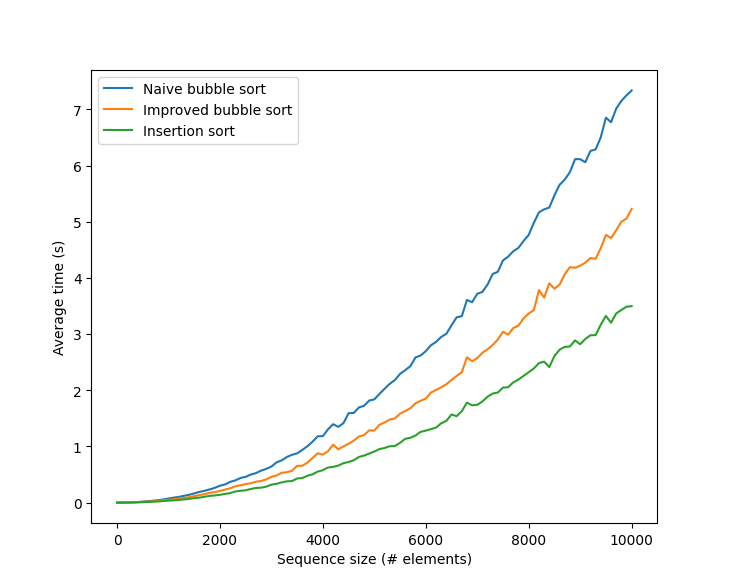
\includegraphics[scale=0.56]{img/plot_reverse_sorted.png}
\vspace{-1em}
\caption{Gráfica comparativa con secuencias ordenadas invertidas}
\label{fig:grafica:invertidas}
\end{figure}

\newpage

La inspección empírica de la gráfica vuelve a revelar que los tres algoritmos siguen una parábola, cumpliendo con el análisis de complejidad. Así mismo, todos los algoritmos tienen un desempeño levemente peor que con secuencias meramente aleatorias. \par

Posteriormente, se realiza la regresión cuadrática y se obtienen los siguientes resultados: \par

\begin{table}[!ht]
\begin{tabular}{|l|r|r|r|r|}
\hline
Algoritmo        & \multicolumn{1}{c|}{$a$} & \multicolumn{1}{c|}{$b$} & \multicolumn{1}{c|}{$c$} & \multicolumn{1}{c|}{$R^2$} \\ \hline
Burbuja inocente & 7.32901e-08            & 1.61687e-05            & -2.53077e-02            & 0.9994136              \\ \hline
Burbuja mejorado & 5.12133e-08            & 1.16794e-05            & -1.69050e-02            & 0.9988019              \\ \hline
Inserción        & 3.50858e-08            & 7.19180e-06            & -1.16396e-02           & 0.9989983              \\ \hline
\end{tabular}
\end{table}

Como se puede observar, todos los algoritmos obtienen un $R^2 > 0,99$. Esto vuelve a representar un ajuste bastante alto mediante la regresión cuadrática. Es posible confirmar que, con secuencias ordenadas invertidas, estos algoritmos tienen una complejidad de $O(|S|^2)$.

\end{document}
